\section{Softwarearchitektur und Design}

\begin{concept}{Grundlagen und Überblick}
\begin{itemize}
    \item \textbf{Business Analyse:}
    \begin{itemize}
        \item Domänenmodell und Kontextdiagramm
        \item Requirements (funktional und nicht-funktional)
        \item Vision und Stakeholder
    \end{itemize}
    
    \item \textbf{Architektur:}
    \begin{itemize}
        \item Logische Struktur des Systems
        \item Technische Konzeption
        \item Qualitätsanforderungen
    \end{itemize}
    
    \item \textbf{Entwicklung:}
    \begin{itemize}
        \item Use Case / User Story Realisierung
        \item Design-Klassendiagramm (DCD)
        \item Implementierung und Tests
    \end{itemize}
\end{itemize}
Architektur und Design sind eng verzahnt und bauen aufeinander auf:
\begin{itemize}
    \item Architektur definiert das "große Ganze"
    \item Design spezifiziert die Details der Umsetzung
    \item Beides basiert auf Requirements und führt zur Implementation
\end{itemize}
%todo: better resolution image
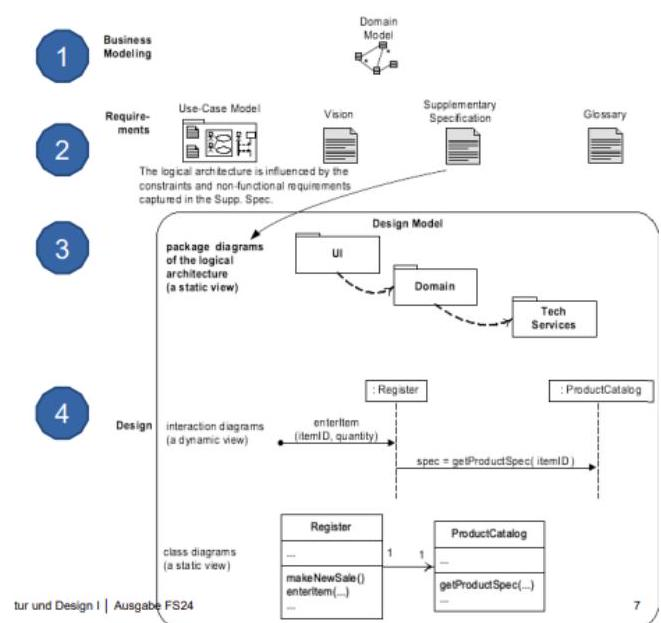
\includegraphics[width=\linewidth]{images/2024_12_29_0d1d7b5551ea1b4b41bdg-07(2)}
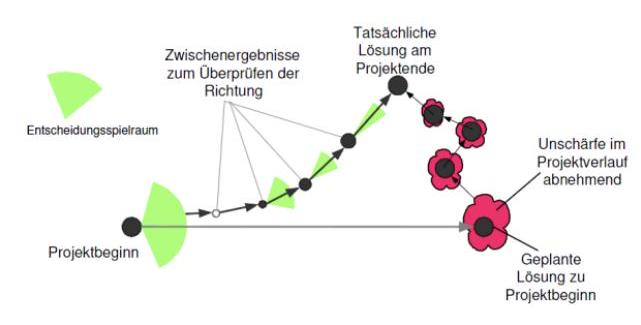
\includegraphics[width=\linewidth]{images/2024_12_29_0d1d7b5551ea1b4b41bdg-08(1)}
\end{concept}

\begin{definition}{Softwarearchitektur}
Die Architektur eines Softwaresystems definiert:

\begin{itemize}
    \item \textbf{Grundlegende Entscheidungen:}
    \begin{itemize}
        \item Programmiersprachen und Plattformen
        \item Aufteilung in Teilsysteme und Komponenten
        \item Schnittstellen zwischen Komponenten
    \end{itemize}
    
    \item \textbf{Strukturelle Aspekte:}
    \begin{itemize}
        \item Verantwortlichkeiten der Teilsysteme
        \item Abhängigkeiten zwischen Komponenten
        \item Einsatz von Basis-Technologien/Frameworks
    \end{itemize}
    
    \item \textbf{Qualitätsaspekte:}
    \begin{itemize}
        \item Erfüllung nicht-funktionaler Anforderungen
        \item Maßnahmen für Performance, Skalierbarkeit etc.
        \item Fehlertoleranz und Ausfallsicherheit
    \end{itemize}
\end{itemize}
\end{definition}

\begin{concept}{Architektursichten (4+1 View Model)}\\
Verschiedene Perspektiven auf die Architektur:

\begin{itemize}
    \item \textbf{Logical View:} End-User, Functionality
    \begin{itemize}
        \item Funktionalität des Systems
        \item Schichten, Subsysteme, Pakete
        \item Klassen und Schnittstellen
    \end{itemize}
    
    \item \textbf{Process View:} Integrators, Performance, Scalability
    \begin{itemize}
        \item Laufzeitverhalten
        \item Prozesse und Threads
        \item Performance und Skalierung
    \end{itemize}

    \item \textbf{Development View:} Programmers, Software Management
    \begin{itemize}
        \item Implementierungsstruktur
        \item Quellcode-Organisation
        \item Build und Deployment
    \end{itemize}
    
    \item \textbf{Physical View:} System Engineers, Topology, Communications
    \begin{itemize}
        \item Hardware-Topologie
        \item Verteilung der Software
        \item Netzwerkkommunikation
    \end{itemize}
\end{itemize}

    
\textbf{+1: Scenarios:}
    \begin{itemize}
        \item Wichtige Use Cases
        \item Validierung der Architektur
        \item Integration der anderen Views
    \end{itemize}
%todo: better resolution image
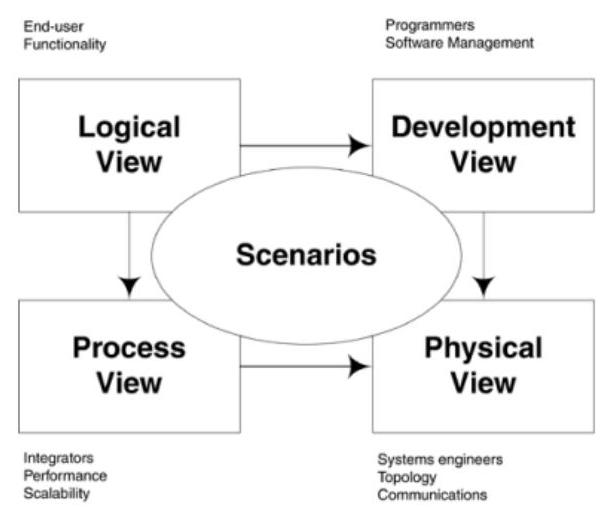
\includegraphics[width=0.9\linewidth]{images/2024_12_29_0d1d7b5551ea1b4b41bdg-09}
\end{concept}

\begin{concept}{Architekturanalyse}\\
erfolgt iterativ mit den Anforderungen (Twin Peaks Model):

\begin{itemize}
    \item \textbf{Anforderungsanalyse:}
    \begin{itemize}
        \item Analyse funktionaler und nicht-funktionaler Anforderungen
        \item Prüfung der Qualität und Stabilität der Anforderungen
        \item Identifikation von Lücken und impliziten Anforderungen
    \end{itemize}
    
    \item \textbf{Architekturentscheidungen:}
    \begin{itemize}
        \item Abstimmung mit Stakeholdern
        \item Berücksichtigung von Randbedingungen
        \item Vorausschauende Planung für zukünftige Änderungen
    \end{itemize}
\end{itemize}

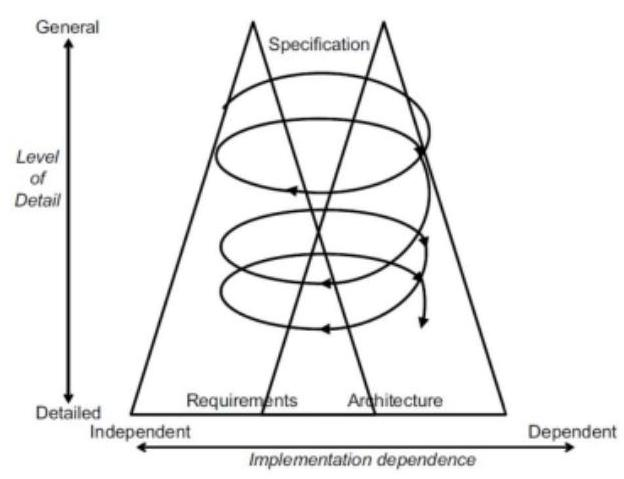
\includegraphics[width=0.9\linewidth]{images/2024_12_29_0d1d7b5551ea1b4b41bdg-08}
\end{concept}

\begin{theorem}{Qualitätsanforderungen}\\
\textbf{ISO 25010:}
\begin{itemize}
    \item Hierarchische Struktur für nicht-funktionale Anforderungen
    \item Definierte Hauptcharakteristiken und Subcharakteristiken
    \item Messbare Metriken für jede Anforderung
    \item Ermöglicht präzise Formulierung und Verifikation
\end{itemize}

\textbf{FURPS+:}
\begin{itemize}
    \item \textbf{F}unctionality (Funktionalität)
    \item \textbf{U}sability (Benutzerfreundlichkeit)
    \item \textbf{R}eliability (Zuverlässigkeit)
    \item \textbf{P}erformance (Leistung)
    \item \textbf{S}upportability (Wartbarkeit)
    \item \textbf{+}: Implementation, Interface, Operations, Packaging, Legal
\end{itemize}
\end{theorem}

\pagebreak

\subsubsection{Designprinzipien und Qualitätskriterien}

\begin{KR}{Clean Architecture}
Prinzipien nach Robert C. Martin:

\textbf{Hauptprinzipien:}
\begin{itemize}
    \item Unabhängigkeit von Frameworks
    \item Testbare Business Rules
    \item Unabhängigkeit von UI
    \item Unabhängigkeit von Datenbank
    \item Unabhängigkeit von externen Systemen
\end{itemize}

\textbf{Schichten (von innen nach außen):}
\begin{enumerate}
    \item Entities (Enterprise Business Rules)
    \item Use Cases (Application Business Rules)
    \item Interface Adapters (Controllers, Presenters)
    \item Frameworks \& Drivers (UI, DB, Devices)
\end{enumerate}

\textbf{Dependency Rule:}
Abhängigkeiten dürfen nur nach innen zeigen.
\end{KR}

\begin{concept}{Architekturprinzipien}
Grundlegende Prinzipien für gute Architektur:

\textbf{Separation of Concerns:}
\begin{itemize}
    \item Trennung von Verantwortlichkeiten
    \item Klare Modulgrenzen
    \item Reduzierte Komplexität
\end{itemize}

\textbf{Information Hiding:}
\begin{itemize}
    \item Kapselung von Implementierungsdetails
    \item Definierte Schnittstellen
    \item Änderbarkeit ohne Seiteneffekte
\end{itemize}

\textbf{Loose Coupling:}
\begin{itemize}
    \item Minimale Abhängigkeiten
    \item Austauschbarkeit
    \item Unabhängige Entwicklung
\end{itemize}
\end{concept}


\begin{corollary}{Qualitätskriterien und deren Umsetzung}\\
Strategien zur Erfüllung von Qualitätsanforderungen:

\textbf{Performance:}
\begin{itemize}
    \item Effiziente Ressourcennutzung (Resource Pooling, Caching)
    \item Optimierte Verarbeitung (Parallelisierung, Lazy Loading)
\end{itemize}

\textbf{Skalierbarkeit:}
\begin{itemize}
    \item Dynamische Anpassung (horizontale/vertikale Skalierung)
    \item Effiziente Lastverteilung (Load Balancing, Partitionierung)
\end{itemize}

\textbf{Wartbarkeit:}
\begin{itemize}
    \item Klare Strukturen (Separation of Concerns, Modularisierung)
    \item Verbesserte Codequalität (Information Hiding, Standardisierung)
\end{itemize}

\textbf{Zuverlässigkeit:}
\begin{itemize}
    \item Fehlerresistenz (Redundanz, Fehlertoleranz)
    \item Prävention und Wiederherstellung (Monitoring, Backup/Recovery)
\end{itemize}

\textbf{Verfügbarkeit:}
\begin{itemize}
    \item Ausfallschutz (Redundanz, Failover-Mechanismen)
    \item Überwachung/Stabilisierung (Health Monitoring, Circuit Breaker)
\end{itemize}

\textbf{Modularität:}
\begin{itemize}
    \item Gut definierte Grenzen (klare Modulgrenzen, hohe Kohäsion)
    \item Minimale Abhängigkeiten zwischen Modulen
\end{itemize}

\textbf{Testbarkeit:}
\begin{itemize}
    \item Einfachheit von Tests (Isolation, Mockbarkeit)
    \item Automatisierung und Skalierung von Tests
\end{itemize}

\textbf{Änderbarkeit:}
\begin{itemize}
    \item Anpassungsfähigkeit (Lokalisierung, Erweiterbarkeit)
    \item Sicherstellung der Kompatibilität (Backward Compatibility)
\end{itemize}

\textbf{Erweiterbarkeit:}
\begin{itemize}
    \item Flexible Architekturen (offene Schnittstellen, Plugin-Systeme)
    \item Serviceorientierung für modulare Erweiterungen
\end{itemize}
\end{corollary}






\begin{concept}{Modulkonzept}\\
Ein Modul (Baustein, Komponente) wird bewertet nach:
\begin{itemize}
    \item \textbf{Kohäsion:} Innerer Zusammenhang
    \item \textbf{Kopplung:} Externe Abhängigkeiten
\end{itemize}

\textbf{Eigenschaften:}
\begin{itemize}
    \item Autarkes Teilsystem
    \item Minimale externe Schnittstellen
    \item Enthält alle benötigten Funktionen/Daten
    \item Verschiedene Formen: Paket, Library, Service
\end{itemize}
\end{concept}

\begin{definition}{Schnittstellen}\\
Module kommunizieren über definierte Schnittstellen:

\begin{itemize}
    \item \textbf{Exportierte Schnittstellen:}
    \begin{itemize}
        \item Definieren angebotene Funktionalität
        \item Vertraglich garantierte Leistungen
        \item Einzige nach außen sichtbare Information
    \end{itemize}
    
    \item \textbf{Importierte Schnittstellen:}
    \begin{itemize}
        \item Von anderen Modulen benötigte Funktionalität
        \item Definieren Abhängigkeiten
        \item Basis für Kopplung
        \item Sollten minimiert werden (Low Coupling)
    \end{itemize}
\end{itemize}
\end{definition}

\subsubsection{Objektorientiertes Design}

\begin{concept}{GRASP Prinzipien}\\
General Responsibility Assignment Software Patterns - Grundlegende Prinzipien für die Zuweisung von Verantwortlichkeiten:

\textbf{Information Expert:}
\begin{itemize}
    \item Zuständigkeit basierend auf Information
    \item Klasse mit relevanten Daten übernimmt Aufgabe
    \item Fördert Kapselung und Kohäsion
\end{itemize}

\textbf{Creator:}
\begin{itemize}
    \item Verantwortung für Objekterstellung
    \item Basierend auf Beziehungen (enthält, aggregiert)
    \item Starke Verwendungsbeziehung
\end{itemize}

\textbf{Controller:}
\begin{itemize}
    \item Koordination von Systemoperationen
    \item Erste Anlaufstelle nach UI
    \item Fassade für Subsystem
\end{itemize}

\textbf{Low Coupling:}
\begin{itemize}
    \item Minimale Abhängigkeiten
    \item Erhöht Wiederverwendbarkeit
    \item Erleichtert Änderungen
\end{itemize}

\textbf{High Cohesion:}
\begin{itemize}
    \item Fokussierte Verantwortlichkeiten
    \item Zusammengehörige Funktionalität
    \item Wartbare Klassen
\end{itemize}
\end{concept}

\begin{concept}{Design nach GRASP}\\
General Responsibility Assignment Software Patterns:

\textbf{Grundprinzipien:}
\begin{itemize}
    \item \textbf{Information Expert:} Verantwortlichkeit dort, wo die Information liegt
    \item \textbf{Creator:} Objekterstellung durch eng verbundene Klassen
    \item \textbf{Controller:} Koordination von Systemoperationen
    \item \textbf{Low Coupling:} Minimale Abhängigkeiten zwischen Klassen
    \item \textbf{High Cohesion:} Starker innerer Zusammenhang in Klassen
\end{itemize}

\textbf{Erweiterte Prinzipien:}
\begin{itemize}
    \item \textbf{Polymorphism:} Typenabhängiges Verhalten durch Polymorphie
    \item \textbf{Pure Fabrication:} Hilfsklassen für besseres Design
    \item \textbf{Indirection:} Vermittler für lose Kopplung
    \item \textbf{Protected Variations:} Kapselung von Änderungen
\end{itemize}
\end{concept}

\begin{concept}{Responsibility Driven Design}\\
Designansatz basierend auf Verantwortlichkeiten und Kollaborationen:

\textbf{Verantwortlichkeiten:}
\begin{itemize}
    \item \textbf{Doing:}
    \begin{itemize}
        \item Aktionen ausführen
        \item Berechnungen durchführen
        \item Andere Objekte steuern
    \end{itemize}
    
    \item \textbf{Knowing:}
    \begin{itemize}
        \item Eigene Daten kennen
        \item Verwandte Objekte kennen
        \item Berechnete Informationen
    \end{itemize}
\end{itemize}

\textbf{Kollaborationen:}
\begin{itemize}
    \item Klare Rollen definieren
    \item Aufgaben verteilen
    \item Interfaces abstimmen
\end{itemize}
\end{concept}

\begin{concept}{Design Pattern Kategorien}\\
Bewährte Lösungsmuster für wiederkehrende Designprobleme:

\textbf{Erzeugungsmuster (Creational):}
\begin{itemize}
    \item Abstract Factory: Familien verwandter Objekte
    \item Factory Method: Objekterzeugung in Subklassen
    \item Singleton: Genau eine Instanz
    \item Builder: Komplexe Objektkonstruktion
    \item Prototype: Klonen existierender Objekte
\end{itemize}

\textbf{Strukturmuster (Structural):}
\begin{itemize}
    \item Adapter: Schnittstellen anpassen
    \item Bridge: Implementation von Abstraktion trennen
    \item Composite: Teil-Ganzes Hierarchien
    \item Decorator: Dynamische Funktionserweiterung
    \item Facade: Vereinfachte Schnittstelle
    \item Proxy: Kontrollierter Zugriff
\end{itemize}

\textbf{Verhaltensmuster (Behavioral):}
\begin{itemize}
    \item Command: Anfrage als Objekt
    \item Observer: Ereignisbenachrichtigung
    \item Strategy: Austauschbare Algorithmen
    \item Template Method: Algorithmus-Skelett
    \item State: Zustandsabhängiges Verhalten
    \item Visitor: Operation zu Objektstruktur hinzufügen
\end{itemize}
\end{concept}

\pagebreak




\subsection{Architekturmuster}

\begin{concept}{Übersicht Architekturmuster}\\
Grundlegende Architekturmuster für Software-Systeme:

\begin{itemize}
    \item \textbf{Layered Pattern:} 
    \begin{itemize}
        \item Strukturierung in horizontale Schichten
        \item Klare Trennung der Verantwortlichkeiten
        \item Abhängigkeiten nur nach unten
    \end{itemize}
    
    \item \textbf{Client-Server Pattern:}
    \begin{itemize}
        \item Verteilung von Diensten
        \item Zentralisierte Ressourcen
        \item Mehrere Clients pro Server
    \end{itemize}
    
    \item \textbf{Master-Slave Pattern:}
    \begin{itemize}
        \item Verteilung von Aufgaben
        \item Zentrale Koordination
        \item Parallelverarbeitung
    \end{itemize}
    
    \item \textbf{Pipe-Filter Pattern:}
    \begin{itemize}
        \item Datenstromverarbeitung
        \item Verkettung von Operationen
        \item Wiederverwendbare Filter
    \end{itemize}
    
    \item \textbf{Broker Pattern:}
    \begin{itemize}
        \item Vermittlung zwischen Komponenten
        \item Entkopplung von Diensten
        \item Zentrale Koordination
    \end{itemize}
    
    \item \textbf{Event-Bus Pattern:}
    \begin{itemize}
        \item Asynchrone Kommunikation
        \item Publisher-Subscriber Modell
        \item Lose Kopplung
    \end{itemize}

    \item \textbf{MVC Pattern:}
    \begin{itemize}
        \item Trennung von Daten, Präsentation und Logik
        \item Wiederverwendbare Komponenten
        \item Klare Strukturierung
    \end{itemize}
\end{itemize}
\end{concept}

\begin{concept}{Schichtenarchitektur (Layered Architecture)}\\
Organisation des Systems in hierarchische Schichten:

\textbf{Typische Schichten:}
\begin{itemize}
    \item Präsentationsschicht (UI)
    \item Anwendungsschicht (Application Logic)
    \item Geschäftslogikschicht (Domain Logic)
    \item Datenzugriffsschicht (Data Access)
\end{itemize}

\textbf{Prinzipien:}
\begin{itemize}
    \item Schichten kommunizieren nur mit direkten Nachbarn
    \item Abhängigkeiten nur nach unten
    \item Jede Schicht kapselt ihre Implementierung
    \item Höhere Schichten sind von unteren abhängig
\end{itemize}

\begin{lstlisting}[language=Java, style=basesmol]
// Praesentationsschicht
public class CustomerController {
    private CustomerService service;
    
    public CustomerDTO getCustomer(String id) {
        return service.findCustomer(id);
    }
}

// Anwendungsschicht
public class CustomerService {
    private CustomerRepository repository;
    
    public CustomerDTO findCustomer(String id) {
        Customer customer = repository.findById(id);
        return CustomerDTO.from(customer);
    }
}

// Geschaeftslogikschicht
public class Customer {
    private CustomerId id;
    private String name;
    
    public void updateName(String newName) {
        validateName(newName);
        this.name = newName;
    }
}

// Datenzugriffsschicht
public class CustomerRepository {
    public Customer findById(String id) {
        // Datenbankzugriff
    }
}
\end{lstlisting}
\end{concept}

\begin{concept}{Clean Architecture}\\
Architektur-Prinzipien nach Robert C. Martin:

\textbf{Hauptprinzipien:}
\begin{itemize}
    \item Unabhängigkeit von Frameworks
    \item Unabhängigkeit von UI
    \item Unabhängigkeit von Datenbank
    \item Testbarkeit ohne externe Systeme
\end{itemize}

\textbf{Schichten (von innen nach außen):}
\begin{itemize}
    \item \textbf{Entities:} 
    \begin{itemize}
        \item Zentrale Geschäftsregeln
        \item Unternehmensweit gültig
        \item Höchste Stabilität
    \end{itemize}
    
    \item \textbf{Use Cases:}
    \begin{itemize}
        \item Anwendungsspezifische Geschäftsregeln
        \item Orchestrierung der Entities
        \item Anwendungslogik
    \end{itemize}
    
    \item \textbf{Interface Adapters:}
    \begin{itemize}
        \item Konvertierung von Daten
        \item Präsentation und Controller
        \item Gateway-Implementierungen
    \end{itemize}
    
    \item \textbf{Frameworks \& Drivers:}
    \begin{itemize}
        \item UI-Framework
        \item Datenbank
        \item Externe Schnittstellen
    \end{itemize}
\end{itemize}

\begin{lstlisting}[language=Java, style=basesmol]
// Entity (innerste Schicht)
public class Customer {
    private CustomerId id;
    private String name;
    
    public void validateName(String name) {
        // Domaenenregeln fuer Namen
    }
}

// Use Case (Business Rules)
public class RegisterCustomerUseCase {
    public void execute(RegisterCustomerCommand cmd) {
        Customer customer = new Customer(cmd.getName());
        customer.validateName(cmd.getName());
        repository.save(customer);
    }
}

// Interface Adapter
public class CustomerController {
    private RegisterCustomerUseCase useCase;
    
    public ResponseEntity<CustomerDTO> register(
            CustomerRequest request) {
        useCase.execute(
            new RegisterCustomerCommand(request.getName())
        );
        return ResponseEntity.ok().build();
    }
}
\end{lstlisting}
\end{concept}

\begin{concept}{Microservices Architektur}\\
Verteilte Architektur mit unabhängigen Services:

\textbf{Charakteristiken:}
\begin{itemize}
    \item Unabhängig entwickelbar und deploybar
    \item Eigene Datenhaltung pro Service
    \item Lose Kopplung
    \item API-basierte Kommunikation
\end{itemize}

\textbf{Patterns:}
\begin{itemize}
    \item Service Discovery
    \item API Gateway
    \item Circuit Breaker
    \item Event Sourcing
    \item CQRS (Command Query Responsibility Segregation)
\end{itemize}

\begin{lstlisting}[language=Java, style=basesmol]
@Service
public class OrderService {
    private final CustomerClient customerClient;
    private final PaymentClient paymentClient;
    
    @CircuitBreaker(name = "order")
    public OrderResult createOrder(OrderRequest request) {
        // Kundeninformationen laden
        CustomerInfo customer = 
            customerClient.getCustomer(request.getCustomerId());
            
        // Zahlungsabwicklung
        PaymentResult payment = 
            paymentClient.processPayment(request.getAmount());
            
        // Order erstellen
        return createOrderWithPayment(customer, payment);
    }
}
\end{lstlisting}
\end{concept}

\begin{concept}{Event-Driven Architecture (EDA)}\\
Architekturstil basierend auf der Erzeugung, Erkennung und Verarbeitung von Events:

\textbf{Kernkomponenten:}
\begin{itemize}
    \item \textbf{Event Producer:} Erzeugt Events
    \item \textbf{Event Channel:} Transportiert Events
    \item \textbf{Event Consumer:} Verarbeitet Events
    \item \textbf{Event Processor:} Transformiert Events
\end{itemize}

\begin{lstlisting}[language=Java, style=basesmol]
// Event Definition
public class OrderCreatedEvent {
    private final OrderId orderId;
    private final CustomerId customerId;
    private final Money totalAmount;
    private final LocalDateTime timestamp;
}

// Event Producer
@Service
public class OrderService {
    private final EventPublisher eventPublisher;
    
    public Order createOrder(OrderRequest request) {
        Order order = orderRepository.save(
            new Order(request));
        
        eventPublisher.publish(new OrderCreatedEvent(
            order.getId(),
            order.getCustomerId(),
            order.getTotalAmount(),
            LocalDateTime.now()
        ));
        
        return order;
    }
}

// Event Consumer
@Service
public class NotificationService {
    @EventListener
    public void handleOrderCreated(
            OrderCreatedEvent event) {
        sendConfirmationEmail(event.getCustomerId());
    }
}
\end{lstlisting}
\end{concept}

\begin{concept}{Integration Patterns}\\
Muster für die Integration verschiedener Systeme:

\textbf{Hauptkategorien:}
\begin{itemize}
    \item \textbf{File Transfer:}
    \begin{itemize}
        \item Datenaustausch über Dateien
        \item Batch-Verarbeitung
        \item Einfache Integration
    \end{itemize}
    
    \item \textbf{Shared Database:}
    \begin{itemize}
        \item Gemeinsame Datenbasis
        \item Direkte Integration
        \item Hohe Kopplung
    \end{itemize}
    
    \item \textbf{Remote Procedure Call:}
    \begin{itemize}
        \item Synchrone Kommunikation
        \item Direkter Methodenaufruf
        \item Service-Orientierung
    \end{itemize}
    
    \item \textbf{Messaging:}
    \begin{itemize}
        \item Asynchrone Kommunikation
        \item Message Broker
        \item Lose Kopplung
    \end{itemize}
\end{itemize}

\textbf{Spezifische Patterns:}
\begin{itemize}
    \item Message Router
    \item Message Translator
    \item Message Filter
    \item Content Enricher
    \item Message Store
\end{itemize}
\end{concept}



\subsection{UML-Modellierung}

\begin{concept}{Grundlagen der UML-Modellierung}\\
UML (Unified Modeling Language) wird im Design auf zwei Arten verwendet:

\textbf{Statische Modelle:}
\begin{itemize}
    \item Struktur des Systems
    \item Klassendiagramme, Paketdiagramme
    \item Fokus auf Pakete, Klassen, Attribute
    \item Keine Methodenimplementierung
\end{itemize}

\textbf{Dynamische Modelle:}
\begin{itemize}
    \item Verhalten des Systems
    \item Sequenz-, Zustands-, Aktivitätsdiagramme
    \item Fokus auf Logik und Verhalten
    \item Methodenimplementierung
\end{itemize}
\end{concept}

\begin{concept}{UML Diagrammtypen}\\
\textbf{Klassendiagramm:}
\begin{itemize}
    \item Klassen mit Attributen und Methoden
    \item Beziehungen zwischen Klassen
    \item Vererbung und Implementierung
    \item Multiplizitäten und Rollen
\end{itemize}

\textbf{Sequenzdiagramm:}
\begin{itemize}
    \item Zeitlicher Ablauf von Interaktionen
    \item Nachrichtenaustausch zwischen Objekten
    \item Synchrone und asynchrone Kommunikation
    \item Alternative Abläufe und Schleifen
\end{itemize}

\textbf{Zustandsdiagramm:}
\begin{itemize}
    \item Zustandsübergänge eines Objekts
    \item Events und Guards
    \item Composite States
    \item Entry/Exit Actions
\end{itemize}

\textbf{Aktivitätsdiagramm:}
\begin{itemize}
    \item Ablauf von Geschäftsprozessen
    \item Kontrollfluss und Datenfluss
    \item Parallelität und Synchronisation
    \item Swimlanes für Verantwortlichkeiten
\end{itemize}
\end{concept}

\begin{concept}{Statische vs. Dynamische Modelle}\\
UML bietet verschiedene Diagrammtypen für unterschiedliche Aspekte:

\textbf{Statische Modelle:}
\begin{itemize}
    \item Fokus auf Struktur und Beziehungen
    \item UML-Klassendiagramm für Klassen, Attribute, Methoden
    \item UML-Paketdiagramm für Modularisierung
    \item UML-Komponentendiagramm für Systembausteine
    \item UML-Verteilungsdiagramm für Deployment
\end{itemize}

\textbf{Dynamische Modelle:}
\begin{itemize}
    \item Fokus auf Verhalten und Interaktion
    \item UML-Sequenzdiagramm für Abläufe
    \item UML-Aktivitätsdiagramm für Prozesse
    \item UML-Zustandsdiagramm für Objektzustände
    \item UML-Kommunikationsdiagramm für Objektkollaborationen
\end{itemize}
\end{concept}

\begin{example2}{UML im Design}\\
\textbf{Klassendiagramm für Order Management:}

\begin{lstlisting}[language=Java, style=basesmol]
public class Order {
    private OrderId id;
    private Customer customer;
    private List<OrderLine> lines;
    private OrderStatus status;
    
    public Money calculateTotal() {
        return lines.stream()
                   .map(OrderLine::getSubTotal)
                   .reduce(Money.ZERO, Money::add);
    }
    
    public void addProduct(Product product, int qty) {
        lines.add(new OrderLine(product, qty));
    }
}

public class OrderLine {
    private Product product;
    private int quantity;
    
    public Money getSubTotal() {
        return product.getPrice()
                     .multiply(quantity);
    }
}

@Service
public class OrderService {
    private OrderRepository repository;
    
    public Order createOrder(OrderRequest request) {
        Order order = new Order(request.getCustomerId());
        request.getItems().forEach(item -> 
            order.addProduct(item.getProduct(), 
                           item.getQuantity()));
        return repository.save(order);
    }
}
\end{lstlisting}
\end{example2}

\begin{example2}{Sequenzdiagramm für Bestellprozess}\\
\textbf{Implementierung einer Bestellverarbeitung:}

\begin{lstlisting}[language=Java, style=basesmol]
@RestController
public class OrderController {
    private final OrderService orderService;
    private final PaymentService paymentService;
    
    public OrderResponse createOrder(
            OrderRequest request) {
        // Validiere Bestellung
        validateOrder(request);
        
        // Erstelle Order
        Order order = orderService.createOrder(request);
        
        // Prozessiere Zahlung
        PaymentResult payment = 
            paymentService.processPayment(
                order.getId(), 
                order.getTotal()
            );
        
        // Update Order Status
        if (payment.isSuccessful()) {
            order.confirm();
            orderService.save(order);
        }
        
        return OrderResponse.from(order);
    }
}
\end{lstlisting}
\end{example2}

\begin{example2}{Zustandsdiagramm für Bestellstatus}\\
\textbf{Implementation des State Patterns:}

\begin{lstlisting}[language=Java, style=basesmol]
public interface OrderState {
    void process(Order order);
    void cancel(Order order);
    void ship(Order order);
}

public class NewOrderState implements OrderState {
    @Override
    public void process(Order order) {
        validateOrder(order);
        order.setState(new ProcessingState());
    }
    
    @Override
    public void cancel(Order order) {
        order.setState(new CancelledState());
    }
    
    @Override
    public void ship(Order order) {
        throw new IllegalStateException(
            "Cannot ship new order");
    }
}

public class Order {
    private OrderState state;
    
    public void process() {
        state.process(this);
    }
    
    void setState(OrderState newState) {
        this.state = newState;
    }
}
\end{lstlisting}
\end{example2}

\begin{KR}{UML Diagrammauswahl}\\
\textbf{Auswahlkriterien:}

\begin{enumerate}
    \item \textbf{Ziel der Modellierung}
    \begin{itemize}
        \item Struktur darstellen -> Klassendiagramm
        \item Abläufe zeigen -> Sequenzdiagramm
        \item Zustände dokumentieren -> Zustandsdiagramm
        \item Prozesse beschreiben -> Aktivitätsdiagramm
    \end{itemize}
    
    \item \textbf{Zielgruppe}
    \begin{itemize}
        \item Entwickler -> detaillierte technische Diagramme
        \item Stakeholder -> vereinfachte Übersichtsdiagramme
        \item Architekten -> Architekturdiagramme
    \end{itemize}
    
    \item \textbf{Detailgrad}
    \begin{itemize}
        \item Überblick -> wenige wichtige Elemente
        \item Detaildesign -> vollständige Details
        \item Implementation -> code-nahe Darstellung
    \end{itemize}
    
    \item \textbf{Phase im Projekt}
    \begin{itemize}
        \item Analyse -> konzeptuelle Modelle
        \item Design -> Designmodelle
        \item Implementation -> detaillierte Modelle
    \end{itemize}
\end{enumerate}
\end{KR}

\begin{example2}{Aktivitätsdiagramm für Geschäftsprozess}\\
\textbf{Implementation eines Workflow:}

\begin{lstlisting}[language=Java, style=basesmol]
public class OrderProcessor {
    public void processOrder(Order order) {
        // Parallel processing
        CompletableFuture.allOf(
            validateInventory(order),
            validatePayment(order)
        ).thenRun(() -> {
            if (order.isValid()) {
                fulfillOrder(order);
            } else {
                handleValidationFailure(order);
            }
        });
    }
    
    private CompletableFuture<Void> validateInventory(
            Order order) {
        return CompletableFuture.runAsync(() -> {
            order.getItems().forEach(item -> {
                if (!inventoryService.isAvailable(item)) {
                    throw new OutOfStockException(item);
                }
            });
        });
    }
}
\end{lstlisting}
\end{example2}

\pagebreak

\subsubsection{Gesamter Architekturprozess}

\begin{KR}{Gesamter Architekturprozess}\\
\textbf{1. Initiale Phase}
\begin{itemize}
    \item Architekturanalyse durchführen
    \item Grundlegende Entscheidungen treffen
    \item Ersten Entwurf erstellen
\end{itemize}

\textbf{2. Iterative Verfeinerung}
\begin{itemize}
    \item Review durchführen
    \item Evaluation vornehmen
    \item Anpassungen basierend auf Feedback
\end{itemize}

\textbf{3. Kontinuierliche Verbesserung}
\begin{itemize}
    \item Regelmäßige Reviews
    \item Neue Anforderungen einarbeiten
    \item Technische Schulden adressieren
\end{itemize}

\textbf{4. Dokumentation}
\begin{itemize}
    \item Entscheidungen festhalten
    \item Architektur dokumentieren
    \item Änderungen nachverfolgen
\end{itemize}

\textbf{5. Qualitätssicherung}
\begin{itemize}
    \item Architektur-Konformität prüfen
    \item Performance-Tests durchführen
    \item Sicherheitsaudits durchführen
\end{itemize}
\end{KR}

\begin{definition}{Architekturprozess-Komponenten}\\
\textbf{Architekturanalyse:}
\begin{itemize}
    \item Erster Schritt im Architekturprozess
    \item Analyse der funktionalen und nicht-funktionalen Anforderungen
    \item Identifikation von Qualitätszielen
    \item Parallel zur Anforderungserhebung (Twin Peaks)
\end{itemize}

\textbf{Architektur-Entscheidungen:}
\begin{itemize}
    \item Konkrete Beschlüsse basierend auf der Analyse
    \item Technologiewahl und Strukturierung
    \item Dokumentation und Begründung
    \item Einschließlich verworfener Alternativen
\end{itemize}

\textbf{Architektur-Entwurf:}
\begin{itemize}
    \item Praktischer Gestaltungsprozess
    \item Anwendung von Architekturmustern
    \item Umsetzung von Qualitätsanforderungen
    \item Erstellung konkreter Artefakte
\end{itemize}

\textbf{Architektur-Review:}
\begin{itemize}
    \item Systematische Überprüfung
    \item Meist durch externe Experten
    \item Prüfung der Anforderungserfüllung
    \item Identifikation von Schwachstellen
\end{itemize}

\textbf{Architektur-Evaluation:}
\begin{itemize}
    \item Bewertung anhand definierter Kriterien
    \item Quantitative und qualitative Analyse
    \item Szenario-basierte Prüfung
    \item Bewertung von Qualitätsattributen
\end{itemize}
\end{definition}


\begin{KR}{Architekturanalyse}\\
\textbf{1. Anforderungen sammeln}
\begin{itemize}
    \item Funktionale Anforderungen gruppieren
    \item Nicht-funktionale Anforderungen identifizieren
    \item Randbedingungen dokumentieren
\end{itemize}

\textbf{2. Qualitätsziele definieren}
\begin{itemize}
    \item Messbare Kriterien festlegen
    \item Priorisierung vornehmen
    \item Trade-offs identifizieren
\end{itemize}

\textbf{3. Einflussfaktoren analysieren}
\begin{itemize}
    \item Technische Faktoren
    \item Organisatorische Faktoren
    \item Wirtschaftliche Faktoren
\end{itemize}
\end{KR}

\begin{KR}{Architektur-Entscheidungen}\\
\textbf{1. Alternativen identifizieren}
\begin{itemize}
    \item Mögliche Lösungen sammeln
    \item Vor- und Nachteile analysieren
    \item Machbarkeit prüfen
\end{itemize}

\textbf{2. Bewertungskriterien}
\begin{itemize}
    \item Erfüllung der Anforderungen
    \item Technische Umsetzbarkeit
    \item Kosten und Aufwand
\end{itemize}

\textbf{3. Entscheidung dokumentieren}
\begin{itemize}
    \item Begründung
    \item Konsequenzen
    \item Verworfene Alternativen
\end{itemize}
\end{KR}

\begin{KR}{Architektur-Entscheidungen dokumentieren}\\
\textbf{1. Entscheidung festhalten}
\begin{itemize}
    \item Dokumentation der getroffenen Architekturentscheidungen
    \item Begründungen und Alternativen
    \item Auswirkungen und Konsequenzen
\end{itemize}

\textbf{2. Strukturierte Dokumentation}
\begin{itemize}
    \item Einheitliches Format für alle Entscheidungen
    \item Verwendung von Templates
    \item Nachvollziehbare Historie der Entscheidungen
\end{itemize}

\textbf{3. Kommunikation}
\begin{itemize}
    \item Regelmäßige Updates an Stakeholder
    \item Transparenz über getroffene Entscheidungen
    \item Einbindung des gesamten Teams
\end{itemize}

\textbf{4. Review und Anpassung}
\begin{itemize}
    \item Regelmäßige Überprüfung der Entscheidungen
    \item Anpassung bei geänderten Rahmenbedingungen
    \item Lessons Learned dokumentieren
\end{itemize}
\end{KR}


\begin{KR}{Architekturentwurf}\\
\textbf{Schritte:}
\begin{enumerate}
    \item Anforderungen analysieren
    \item Architekturstil wählen
    \item Module identifizieren
    \item Schnittstellen definieren
    \item Mit Stakeholdern abstimmen
\end{enumerate}

\textbf{Qualitätskriterien:}
\begin{itemize}
    \item Änderbarkeit
    \item Wartbarkeit
    \item Erweiterbarkeit
    \item Testbarkeit
\end{itemize}
\end{KR}

\begin{KR}{Architektur-Review durchführen}\\
\textbf{Vorgehen:}
\begin{enumerate}
    \item \textbf{Vorbereitung}
    \begin{itemize}
        \item Architektur-Dokumentation zusammenstellen
        \item Review-Team zusammenstellen
        \item Checklisten vorbereiten
    \end{itemize}
    
    \item \textbf{Durchführung}
    \begin{itemize}
        \item Architektur vorstellen
        \item Anforderungen prüfen
        \item Entscheidungen hinterfragen
        \item Risiken identifizieren
    \end{itemize}
    
    \item \textbf{Nachbereitung}
    \begin{itemize}
        \item Findings dokumentieren
        \item Maßnahmen definieren
        \item Follow-up planen
    \end{itemize}
\end{enumerate}

\textbf{Prüfkriterien:}
\begin{itemize}
    \item Anforderungserfüllung
    \item Technische Machbarkeit
    \item Zukunftssicherheit
    \item Best Practices
\end{itemize}
\end{KR}



\begin{KR}{Architektur-Evaluation}\\
Systematische Bewertung einer Softwarearchitektur:

\textbf{1. Qualitätsattribute identifizieren}
\begin{itemize}
    \item Performance
    \item Skalierbarkeit
    \item Wartbarkeit
    \item Sicherheit
\end{itemize}

\textbf{2. Szenarien entwickeln}
\begin{itemize}
    \item Normale Nutzung
    \item Grenzfälle
    \item Fehlerfälle
    \item Wartungsszenarien
\end{itemize}

\textbf{3. Architektur analysieren}
\begin{itemize}
    \item Strukturanalyse
    \item Verhaltensanalyse
    \item Trade-off Analyse
\end{itemize}

\textbf{4. Risiken identifizieren}
\begin{itemize}
    \item Technische Risiken
    \item Geschäftsrisiken
    \item Architekturrisiken
\end{itemize}
\end{KR}

\columnbreak

\subsubsection{Beispiele}

\begin{example2}{Typische Prüfungsaufgabe: Architekturanalyse und Entscheidungen}\\
\textbf{Aufgabenstellung:}
Analysieren Sie folgende Anforderungen und leiten Sie architektonische Konsequenzen ab:
\begin{itemize}
    \item System muss 24/7 verfügbar sein
    \item 10.000 gleichzeitige Benutzer
    \item Reaktionszeit unter 1 Sekunde
    \item Jährliche Wartungsfenster maximal 4 Stunden
\end{itemize}

\textbf{Lösung:}
\begin{itemize}
    \item \textbf{Architekturentscheidungen:}
    \begin{itemize}
        \item Verteilte Architektur für Hochverfügbarkeit
        \item Load Balancing für gleichzeitige Benutzer
        \item Caching-Strategien für Performanz
        \item Blue-Green Deployment für Wartung
    \end{itemize}
    
    \item \textbf{Begründungen:}
    \begin{itemize}
        \item Verteilung minimiert Single Points of Failure
        \item Load Balancer verteilt Last gleichmäßig
        \item Caching reduziert Datenbankzugriffe
        \item Blue-Green erlaubt Updates ohne Downtime
    \end{itemize}
\end{itemize}
\end{example2}

\begin{example2}{Architekturentwurf}\\
\textbf{Aufgabe:} Entwerfen Sie die grundlegende Architektur für ein Online-Banking-System.

\textbf{Lösung:}
\begin{itemize}
    \item \textbf{Anforderungsanalyse:}
    \begin{itemize}
        \item Sicherheit (ISO 25010)
        \item Performance (FURPS+)
        \item Skalierbarkeit
    \end{itemize}
    
    \item \textbf{Architekturentscheidungen:}
    \begin{itemize}
        \item Mehrschichtige Architektur
        \item Microservices für Skalierbarkeit
        \item Sicherheitsschicht
    \end{itemize}
    
    \item \textbf{Module:}
    \begin{itemize}
        \item Authentifizierung
        \item Transaktionen
        \item Kontoführung
    \end{itemize}
\end{itemize}
\end{example2}

\subsection{other examples}

\begin{example2}{Gute Testbarkeit}\\

\begin{lstlisting}[language=Java, style=basesmol]
public class OrderService {
    private final OrderRepository repository;
    private final PaymentGateway paymentGateway;
    
    // Dependency Injection ermoeglicht einfaches Mocking
    public OrderService(
            OrderRepository repository,
            PaymentGateway paymentGateway) {
        this.repository = repository;
        this.paymentGateway = paymentGateway;
    }
    
    // Klare Methoden-Verantwortlichkeiten
    public OrderResult createOrder(OrderRequest request) {
        validateRequest(request);
        Order order = createOrderEntity(request);
        PaymentResult payment = processPayment(order);
        return createOrderResult(order, payment);
    }
}
\end{lstlisting}
\end{example2}

\subsubsection{Dokumentation Architektur}

\begin{example2}{Architekturanalyse}\\
\textbf{Analyse für ein E-Commerce-System:}

\begin{lstlisting}[language=Java, style=basesmol]
// Dokumentation der Analyse
public class ArchitectureAnalysis {
    public class QualityRequirement {
        String name;
        String description;
        int priority;
        String measurementCriteria;
    }
    
    public class ArchitecturalConstraint {
        String type; // Technical, Organizational, Business
        String description;
        String impact;
    }
    
    // Beispiel Qualitaetsanforderung
    QualityRequirement performance = new QualityRequirement(
        "Response Time",
        "System responses within 200ms",
        1,
        "95th percentile < 200ms"
    );
    
    // Beispiel Randbedingung
    ArchitecturalConstraint technology = new ArchitecturalConstraint(
        "Technical",
        "Must use Java 17",
        "Affects framework selection"
    );
}
\end{lstlisting}
\end{example2}

\begin{example2}{Architektur-Entscheidungen}\\
\textbf{Entscheidungsdokumentation:}

\begin{lstlisting}[language=Java, style=basesmol]
public class ArchitectureDecision {
    String id;
    String title;
    String context;
    String decision;
    String rationale;
    List<String> consequences;
    List<Alternative> alternatives;
    
    class Alternative {
        String description;
        List<String> pros;
        List<String> cons;
        String rejectionReason;
    }
}

// Beispiel:
ArchitectureDecision caching = new ArchitectureDecision(
    "AD001",
    "Caching Strategy",
    "High read load on product catalog",
    "Use Redis as distributed cache",
    "Better performance and scalability",
    List.of("Requires Redis expertise", 
            "Additional infrastructure"),
    List.of(new Alternative(
        "In-memory cache",
        List.of("Simple", "No additional infrastructure"),
        List.of("Not distributed", "Memory limited"),
        "Doesn't scale horizontally"
    ))
);
\end{lstlisting}
\end{example2}

\begin{example2}{Architektur-Review}\\
\textbf{Review-Protokoll:}

\begin{lstlisting}[language=Java, style=basesmol]
public class ArchitectureReview {
    public class Finding {
        String area;
        String observation;
        Risk risk;
        String recommendation;
        Priority priority;
    }
    
    public class Action {
        String description;
        String responsible;
        LocalDate dueDate;
        Status status;
    }
    
    List<Finding> findings = List.of(
        new Finding(
            "Security",
            "Missing rate limiting",
            Risk.HIGH,
            "Implement API gateway with rate limiting",
            Priority.HIGH
        )
    );
    
    List<Action> actions = List.of(
        new Action(
            "Implement API gateway",
            "Team A",
            LocalDate.now().plusWeeks(2),
            Status.OPEN
        )
    );
}
\end{lstlisting}
\end{example2}